\documentclass{article}
\usepackage{amsfonts,enumerate,zed-csp}
\usepackage{graphicx}
%%%%%%%%%%%%%%%%%%%%%%%%%%%%%%%%%%%%%%%%%%%%%%%%%%%%%%%%%%%%%%%%
%  6.826 (POCS Seminar) macro file for handouts and problem sets.
%
% You should save this file as handout.tex
%
% Your main LaTeX file should look like this:
%
%        \documentstyle[12pt]{article}
%
%        %%%%%%%%%%%%%%%%%%%%%%%%%%%%%%%%%%%%%%%%%%%%%%%%%%%%%%%%%%%%%%%%
%  6.826 (POCS Seminar) macro file for handouts and problem sets.
%
% You should save this file as handout.tex
%
% Your main LaTeX file should look like this:
%
%        \documentstyle[12pt]{article}
%
%        %%%%%%%%%%%%%%%%%%%%%%%%%%%%%%%%%%%%%%%%%%%%%%%%%%%%%%%%%%%%%%%%
%  6.826 (POCS Seminar) macro file for handouts and problem sets.
%
% You should save this file as handout.tex
%
% Your main LaTeX file should look like this:
%
%        \documentstyle[12pt]{article}
%
%        \input{handout}
%%%%%%%%%%%%%%%%%%%%%%%%%%%%%%%%%%%%%%%%%%%%%%%%%%%%%%%%%%%%%%%%

\oddsidemargin 0in
\evensidemargin 0in
\marginparwidth 40pt
\marginparsep 10pt
\topmargin 0pt
\headsep 0in
\headheight 0in
\textheight 8.5in
\textwidth 6in
\brokenpenalty=10000

% \handout{number}{date}{title}

\newcommand{\handout}[3]{


\begin{center}
\rule{\textwidth}{.0075in} \\
\rule[3mm]{\textwidth}{.0075in}\\

CMU 17-651\hfill Models of Software Systems\hfill Fall 2018\\[3ex]

{\Large\bf #3}\\[3ex]

Dario A Lencina-Talarico \hfill {\bf Handout #1} \hfill #2

\rule{\textwidth}{.0075in} \\
\rule[3mm]{\textwidth}{.0075in} \\
\end{center}

}

% \homework{number}{date}{title}{due-date}
\newcommand{\homework}[4]{

\begin{center}
\rule{\textwidth}{.0075in} \\
\rule[3mm]{\textwidth}{.0075in}\\

CMU 17-651\hfill Models of Software Systems\hfill Fall 2018\\[3ex]

{\Large\bf #3} \\[3ex]

Dario A Lencina Talarico \hfill  #1  \hfill Due: #2\\

\rule{\textwidth}{.0075in} \\
\rule[3mm]{\textwidth}{.0075in} \\
\end{center}

%\noindent
%{\bf Due date: #4}

}

% \solutionset{number}{date}{title}{due-date}
\newcommand{\solutionset}[4]{

\begin{center}
\rule{\textwidth}{.0075in} \\
\rule[3mm]{\textwidth}{.0075in}\\

CMU 17-651\hfill Models of Software Systems\hfill Fall 2016\\[3ex]

{\Large\bf #3} \\[3ex]

Garlan  \hfill  Solutions for Homework #1  \hfill  #2\\

\rule{\textwidth}{.0075in} \\
\rule[3mm]{\textwidth}{.0075in} \\
\end{center}

%\noindent
%{\bf Due date: #4}

}

% \problem{problem-number}
\newcommand{\problem}[1]{
\vspace{2ex}
\noindent
{\bf Problem #1.}

}

% \solution{solution-number}{points}
\newcommand{\solution}[2]{
\vspace{3ex}
\noindent
{\bf Problem #1}  (#2 points)

}

\newcommand{\cscomment}{
\vspace{1ex}
\noindent Comments: }

% \parts{part-alphabet}{points}
\newcommand{\parts}[2]{
\vspace{2ex}
\noindent
{\bf (#1)}  (#2 points)

}

% \problems{problems-number}{points}
\newcommand{\problems}[2]{
\vspace{3ex}
\noindent
{\bf Problem #1}  (#2 points)

}

\newenvironment{symbolfootnotes}{\def\thefootnote{\fnsymbol{footnote}}}{}

%%%%%%%%%%%%%%%%%%%%%%%%%%%%%%%%%%%%%%%%%%%%%%%%%%%%%%%%%%%%%%%%

\oddsidemargin 0in
\evensidemargin 0in
\marginparwidth 40pt
\marginparsep 10pt
\topmargin 0pt
\headsep 0in
\headheight 0in
\textheight 8.5in
\textwidth 6in
\brokenpenalty=10000

% \handout{number}{date}{title}

\newcommand{\handout}[3]{


\begin{center}
\rule{\textwidth}{.0075in} \\
\rule[3mm]{\textwidth}{.0075in}\\

CMU 17-651\hfill Models of Software Systems\hfill Fall 2018\\[3ex]

{\Large\bf #3}\\[3ex]

Dario A Lencina-Talarico \hfill {\bf Handout #1} \hfill #2

\rule{\textwidth}{.0075in} \\
\rule[3mm]{\textwidth}{.0075in} \\
\end{center}

}

% \homework{number}{date}{title}{due-date}
\newcommand{\homework}[4]{

\begin{center}
\rule{\textwidth}{.0075in} \\
\rule[3mm]{\textwidth}{.0075in}\\

CMU 17-651\hfill Models of Software Systems\hfill Fall 2018\\[3ex]

{\Large\bf #3} \\[3ex]

Dario A Lencina Talarico \hfill  #1  \hfill Due: #2\\

\rule{\textwidth}{.0075in} \\
\rule[3mm]{\textwidth}{.0075in} \\
\end{center}

%\noindent
%{\bf Due date: #4}

}

% \solutionset{number}{date}{title}{due-date}
\newcommand{\solutionset}[4]{

\begin{center}
\rule{\textwidth}{.0075in} \\
\rule[3mm]{\textwidth}{.0075in}\\

CMU 17-651\hfill Models of Software Systems\hfill Fall 2016\\[3ex]

{\Large\bf #3} \\[3ex]

Garlan  \hfill  Solutions for Homework #1  \hfill  #2\\

\rule{\textwidth}{.0075in} \\
\rule[3mm]{\textwidth}{.0075in} \\
\end{center}

%\noindent
%{\bf Due date: #4}

}

% \problem{problem-number}
\newcommand{\problem}[1]{
\vspace{2ex}
\noindent
{\bf Problem #1.}

}

% \solution{solution-number}{points}
\newcommand{\solution}[2]{
\vspace{3ex}
\noindent
{\bf Problem #1}  (#2 points)

}

\newcommand{\cscomment}{
\vspace{1ex}
\noindent Comments: }

% \parts{part-alphabet}{points}
\newcommand{\parts}[2]{
\vspace{2ex}
\noindent
{\bf (#1)}  (#2 points)

}

% \problems{problems-number}{points}
\newcommand{\problems}[2]{
\vspace{3ex}
\noindent
{\bf Problem #1}  (#2 points)

}

\newenvironment{symbolfootnotes}{\def\thefootnote{\fnsymbol{footnote}}}{}

%%%%%%%%%%%%%%%%%%%%%%%%%%%%%%%%%%%%%%%%%%%%%%%%%%%%%%%%%%%%%%%%

\oddsidemargin 0in
\evensidemargin 0in
\marginparwidth 40pt
\marginparsep 10pt
\topmargin 0pt
\headsep 0in
\headheight 0in
\textheight 8.5in
\textwidth 6in
\brokenpenalty=10000

% \handout{number}{date}{title}

\newcommand{\handout}[3]{


\begin{center}
\rule{\textwidth}{.0075in} \\
\rule[3mm]{\textwidth}{.0075in}\\

CMU 17-651\hfill Models of Software Systems\hfill Fall 2018\\[3ex]

{\Large\bf #3}\\[3ex]

Dario A Lencina-Talarico \hfill {\bf Handout #1} \hfill #2

\rule{\textwidth}{.0075in} \\
\rule[3mm]{\textwidth}{.0075in} \\
\end{center}

}

% \homework{number}{date}{title}{due-date}
\newcommand{\homework}[4]{

\begin{center}
\rule{\textwidth}{.0075in} \\
\rule[3mm]{\textwidth}{.0075in}\\

CMU 17-651\hfill Models of Software Systems\hfill Fall 2018\\[3ex]

{\Large\bf #3} \\[3ex]

Dario A Lencina Talarico \hfill  #1  \hfill Due: #2\\

\rule{\textwidth}{.0075in} \\
\rule[3mm]{\textwidth}{.0075in} \\
\end{center}

%\noindent
%{\bf Due date: #4}

}

% \solutionset{number}{date}{title}{due-date}
\newcommand{\solutionset}[4]{

\begin{center}
\rule{\textwidth}{.0075in} \\
\rule[3mm]{\textwidth}{.0075in}\\

CMU 17-651\hfill Models of Software Systems\hfill Fall 2016\\[3ex]

{\Large\bf #3} \\[3ex]

Garlan  \hfill  Solutions for Homework #1  \hfill  #2\\

\rule{\textwidth}{.0075in} \\
\rule[3mm]{\textwidth}{.0075in} \\
\end{center}

%\noindent
%{\bf Due date: #4}

}

% \problem{problem-number}
\newcommand{\problem}[1]{
\vspace{2ex}
\noindent
{\bf Problem #1.}

}

% \solution{solution-number}{points}
\newcommand{\solution}[2]{
\vspace{3ex}
\noindent
{\bf Problem #1}  (#2 points)

}

\newcommand{\cscomment}{
\vspace{1ex}
\noindent Comments: }

% \parts{part-alphabet}{points}
\newcommand{\parts}[2]{
\vspace{2ex}
\noindent
{\bf (#1)}  (#2 points)

}

% \problems{problems-number}{points}
\newcommand{\problems}[2]{
\vspace{3ex}
\noindent
{\bf Problem #1}  (#2 points)

}

\newenvironment{symbolfootnotes}{\def\thefootnote{\fnsymbol{footnote}}}{}

\newcommand{\Until}{\,\mathcal{U}\,}
\newcommand{\Next}{\bigcirc}
\begin{document}

\homework{}{7 November 2016}{Homework \#11: Concurrency Modeling and LTL}{}

\begin{enumerate}
\item Exercises from MK06. ({\sc Note}: For every question in which you are asked to use LTSA, you should include the relevant output of the checker and briefly explain those results.)
\begin{enumerate}
\item 5.4 (just the FSP part)
  The Dining Savages: A tribe of savages eats communal dinners from a large pot that can hold M servings of stewed missionary. When a savage wants to eat, he helps himself from the pot unless it is empty in which case he waits for the pot to be filled. If the pot is empty, the cook refills the pot with M servings. The behavior of the savages and the cook is described by:
  \begin{verbatim}
  SAVAGE = (getserving -> SAVAGE).
  COOK   = (fillpot -> COOK).
  \end{verbatim}
  Model the behavior of the pot as an FSP process and then implement it as a Java monitor. \\
  \\
  \begin{verbatim}
  const PotCapacity = 5
  range Int = 0..PotCapacity

  SAVAGE = (getserving -> SAVAGE).

  COOK   = (fillpot -> COOK).

  POT(I=0) = POTIMP[I],
  POTIMP[n:Int] = (when(n > 0) getserving -> POTIMP[n-1]
                  |when(n == 0) fillpot -> POTIMP[PotCapacity]
                  ).

  ||FEAST(N=5) = (forall [i:1..N] savage[i]:SAVAGE || COOK || POT(PotCapacity))
                 /{{savage[1..N]}.getserving/getserving}.
  \end{verbatim}
\item 6.2
  One solution to the Dining Philosophers problem permits only four philosophers to sit down at the table at the same time. Specify a BUTLER process which, when composed with the model of section 6.2, permits a maximum of four philosophers to engage in the sitdown action before an arise action occurs. Show that this system is deadlock-free.
\begin{verbatim}
const N = 5

PHIL = (butler.requestSitdown->right.get->left.get
               ->eat->left.put->right.put
               -> butler.arise->PHIL).

FORK = (get -> put -> FORK).

BUTLER = BUTLER[0],
BUTLER[n:0..(N-1)] =(when (n<(N-1)) requestSitdown -> BUTLER[n+1]
|arise -> BUTLER[n-1]).

||DINERS =
        (forall [i:0..N-1] phil[i]:PHIL || {phil[i:0..(N - 1)]}::butler:BUTLER
        || forall [i:0..N-1] {phil[i].left,phil[((i-1)+N)%N].right}::FORK
        ).  
\end{verbatim}
\item 6.4
  It is possible for the following system to deadlock. Explain how this deadlock occurs and relate it to one of the four necessary and sufficient conditions for deadlock to occur.
    \begin{verbatim}
    Alice = (call.bob -> wait.chris -> Alice).
    Bob   = (call.chris -> wait.alice -> Bob).
    Chris = (call.alice -> wait.bob -> Chris).

    ||S = (Alice || Bob || Chris) /{call/wait}.
\end{verbatim}
    Given that the label rewrite maps all the calls to the wait prefixes, that means that the system can be rewriten as:
    \begin{verbatim}
    Alice = (bob -> chris -> Alice).
    Bob   = (chris -> alice -> Bob).
    Chris = (alice -> bob -> Chris).

    ||S = (Alice || Bob || Chris).
\end{verbatim}
    It can be seen that Alice tries to execute bob, but because Chris also defines an action called bob, then Alice gets stuck.
    Chris can not make any progress either as it is waiting for Bob to get to the alice action, and Bob is waiting for Alice to get to the chris action. \\
    \\
    In my opinion, this is an example of ``Wait-for-cycle'': ``a circular chain (or cycle) of processes exists such that each process holds a resource which its successor in the cycle is waiting to acquire.''[MK06]\\
    \\
The following model attempts to fix the problem by allowing Alice, Bob and Chris to time out from a call attempt. Is a deadlock still possible? If so, describe how the deadlock can occur and give an execution trace leading to the deadlock.

\begin{verbatim}    
Alice = (call.bob -> wait.chris -> Alice          
      |  timeout.alice -> wait.chris ->Alice).    
Bob   = (call.chris -> wait.alice -> Bob          
      |  timeout.bob -> wait.alice ->Bob).    
Chris = (call.alice -> wait.bob -> Chris          
      |  timeout.chris -> wait.bob ->Chris).    

||S = (Alice || Bob || Chris) /{call/wait}.
\end{verbatim}
Yes, it is possible to get a deadlock, using lts I was able to get the following trace:
\begin{verbatim}
Trace to DEADLOCK:
	timeout.alice
	timeout.bob
	timeout.chris
\end{verbatim}
using a sequence = $\langle timeout.alice, timeout.bob, timeout.chris \rangle$ \\
  \item 7.1 
    What action trace violates the following safety property?
    \begin{verbatim}
      property PS = (a->(b->PS|a->PS)|b->a->PS). 
   \end{verbatim}
    $bad\_trace = \langle b, b \rangle$ \\    
  \item 7.2 
    A lift has a maximum capacity of ten people. In the model of the lift control system, passengers entering a lift are signaled by an enter action and passengers leaving the lift are signaled by an exit action. Specify a safety property in FSP which when composed with the lift will check that the system never allows the lift that it controls to have more than ten occupants. \\
\begin{verbatim}
const MAX_PASSENGERS = 100

range Passengers = 0..MAX_PASSENGERS

property RESPECT_OCCUPANCY(N=0) = RESPECT_OCCUPANCY_IMP[N],
RESPECT_OCCUPANCY_IMP[p:Passengers] = (when(p < 10) enter -> RESPECT_OCCUPANCY_IMP[p + 1]
                                      |exit -> RESPECT_OCCUPANCY_IMP[p - 1]
                                      ).
  \end{verbatim}
  \item 7.3 
   Specify a safety property for the car park problem of Chapter 5, which asserts that the car park does not overflow. Specify a progress property which asserts that cars eventually enter the car park. If car departure is lower priority than car arrival, does starvation occur? \\

\begin{verbatim}
const MAX_CAPACITY = 10

property RESPECT_MAX_CAPACITY(N=0) = MAX_CAPACITY_IMP[N],
MAX_CAPACITY_IMP[i:0..N] = (when(i < N) arrive -> MAX_CAPACITY_IMP[i + 1]
                           |when(i > 0) exit -> MAX_CAPACITY_IMP[i - 1] 
                           ).

||CARPARK = (ARRIVALS||CARPARKCONTROL(MAX_CAPACITY)||DEPARTURES || RESPECT_MAX_CAPACITY(0)).
\end{verbatim}
Progress property:
\begin{verbatim}
progress CAR_ARRIVE = {arrive}
\end{verbatim}

After running LTSA progress check:

\begin{verbatim}
Progress Check...
-- States: 11 Transitions: 20 Memory used: 45837K
No progress violations detected.
Progress Check in: 0ms
\end{verbatim}

After decreasing the priority of the depart event, I found that it is not possible for all vehicles to leave:

\begin{verbatim}
||CARPARK = (ARRIVALS||CARPARKCONTROL(MAX_CAPACITY)|| DEPARTURES 
|| RESPECT_MAX_CAPACITY(0)) >> {depart}.
\end{verbatim}

As it can be seen in the screenshot, the depart action is not available even when the parking lot is almost full. \\
\\
I consider that to be a typical case of \textbf{starvation}.

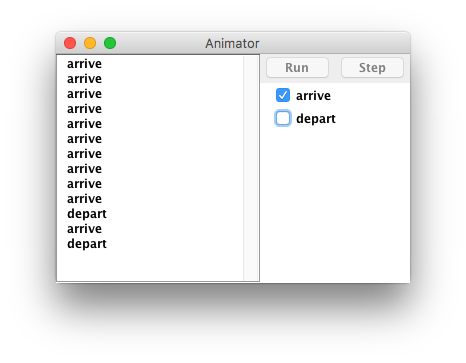
\includegraphics[scale=0.5]{img1.png}

\end{enumerate}

\item Using the semantic rules for LTL covered in the lecture on that topic, expand the following temporal formulas to their equivalent semantic form (using the $(\sigma,i)\models P)$  representation). For each, say what it means in English.
\begin{enumerate}
\item $Q \implies \Diamond \Box P$ \\
  $(\sigma,1)\models Q \implies \Diamond \Box P$ \\
  if initially Q then eventually P will be true forever. \\
  \\
  Procedure: in lecture 19 it is explained what $\Diamond \Box$ means and how the $\implies$
  operations functions as an if statement, I did not have much more procedure than that to attempt to answer this question.
\item $\Diamond (Q \land \Box P)$ \\
  $(\sigma,1)\models \Diamond ( Q \land \Box P)$ \\
  There is a state in the trace where initialy Q and always P are true \\
  \\
  Procedure: it is important to mention that the whole expression is wrapped by a $\Diamond$ operator, this is equivalent to an exists statement in predicate logic, then the expression inside says that initially Q and always P have to be true.
\end{enumerate}
\item Translate each of the following into a formula of linear temporal logic. (\textsc{Note}: For this assignment, use only the temporal logic operators: $\Box$, $\Diamond$, $\Next$, $\Until$, $\Until_w$.)
\begin{enumerate}
\item $p$ is sometimes true and sometimes false. \\
$ \Diamond p \land \Diamond \neg p $
\item $p$ and $q$ are never true together. \\
$ \neg \Diamond ( p \land q) $
\item $q$ and $r$ are both eventually false. \\
$ \neg \Diamond q \land \neg \Diamond r $  
\item $q$ and $r$ are eventually both false. \\
$ \Diamond (\neg q \land \neg r) $  
\item If $p$ is never true, then $q$ is always true. \\
  $\neg p \implies \Box q $ 
\item Eventually, if $p$ is true, then $q$ is also true \\
  $ \Diamond (p \implies q) $
\item If $p$ is eventually true, $q$ is never true. \\
  $ \Diamond p \implies \neg q $
\item $p$ is true finitely often (and at least once). \\
  $\Diamond \Box p$
\item If $p$ is initially true, then it will be true infinitely often; otherwise it will never be true. \\
  $p \implies \Box \Diamond p$ 
\item $p$ is initially true and thereafter alternates between being true and being false (i.e., if $(\sigma,i)\models p$, then $(\sigma,i+1)\models \neg p$ and if $(\sigma,i)\models \neg p$, then $(\sigma,i+1)\models p$). \\
  \\
  $p \land \Next \neg p$
  
\end{enumerate}

\end{enumerate}

\end{document}
